\newpage
\hypertarget{sec:stringRep}{}
\section{A string representation of our learning box}
\label{sec_A string representation of our learning box}
\genHeader

In the next SDM we shall create a string representation for all the contents in a single learning box. To accomplish this, we will have to iterate through 
every card, in every partition. The concept is similar to \texttt{Partition}'s \texttt{empty} method, except we'll need to create a nested \emph{for each}
loop (Fig.~\ref{fig:goal_stringRep}). Further still, we'll need to call a helper method to accumulate the contents of each card to a single string.

\vspace{1cm}

\begin{figure}[htbp]
	\centering
	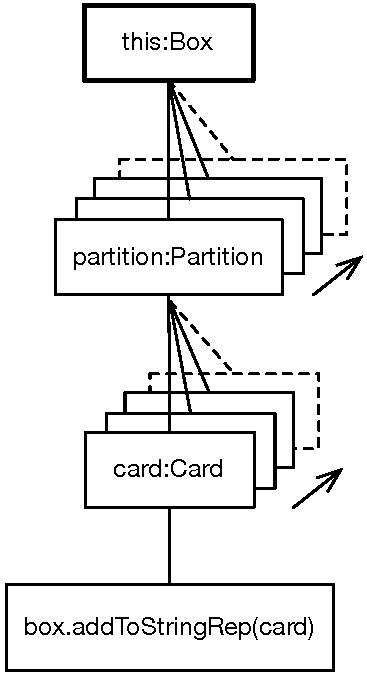
\includegraphics[width=0.3\textwidth]{goal_stringRep.pdf}
	\caption{Nested \emph{For Each} loops}
	\label{fig:goal_stringRep}
\end{figure}

\vspace{1cm}

As you can see, The first loop will match all partitions, while the second matches each card. Finally, a \emph{statement node} is used to invoke the
\texttt{addToStringRep} method. In contrast to how they were used for conditional branching in \texttt{grow}, this statement node will simply invoke a
void method.

Unlike \texttt{initializeBox} however, this helper method is actually better specified as an injection so, analogously to how you implemented
\texttt{deter\-mine\-Next\-Size} for \texttt{box.grow()}, quickly edit \texttt{BoxImpl.java} by replacing the default code for \texttt{addToStringRep} with that
in Fig.~\ref{code:addToStringRep_inject_file}. You can use Eclipse's built-in auto-completion to speed up this process. Save, create the injection file, and
confirm the contents of \texttt{BoxImpl.inject}.

\newpage

\vspace*{3cm}

\begin{figure}[h!]
\centering
\begin{lstlisting}[language=Java, keywordstyle={\bfseries\color{purple}}, backgroundcolor=\color{white}]
public void addToStringRep(Card card) {
	// [user code injected with eMoflon]
	StringBuilder sb = new StringBuilder();
	if (stringRep == null) {
		sb.append("BoxContent: [");
	} else {
		sb.append(stringRep);
		sb.append(", [");
	}
	sb.append(card.getFace());
	sb.append(", ");
	sb.append(card.getBack());
	sb.append("]");
	stringRep = sb.toString();
	}
        \end{lstlisting}
        \caption{Implementation of \texttt{addToStringRep}}
        \label{code:addToStringRep_inject_file}
    \end{figure}
    \FloatBarrier

\newpage
\hypertarget{stringRep vis}{}
\subsection{Implementing stringRep}
\visHeader

\begin{itemize}

\item[$\blacktriangleright$] Visual SDMs support arbitrary nesting of \emph{for each} story nodes via special guards. In \hyperlink{emptyPartition vis}{section
5.1} we used the \texttt{[end]} edge guard to terminate a loop. Now we'll use a new guard, the \texttt{[each time]}\define{[each time]} guard, to indicate control flow that is \emph{nested} and
executed for each match. Go ahead and create the SDM for \texttt{Box::toString} until it closely resembles Fig.~\ref{fig:sdm_tostring_1}. 

\vspace{0.5cm}

\begin{figure}[htbp]
\begin{center}
  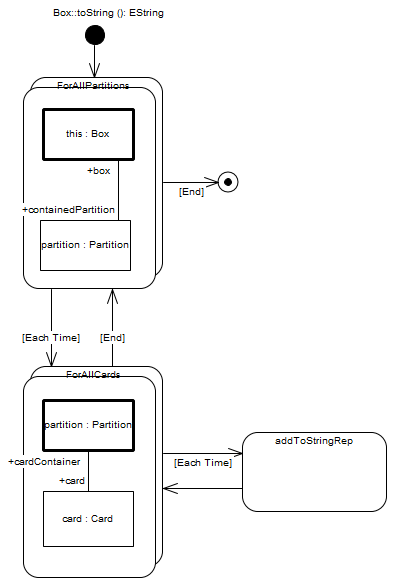
\includegraphics[width=0.8\textwidth]{ea_toStringStart}
  \caption{Control flow with nested loops} 
  \label{fig:sdm_tostring_1}
\end{center}
\end{figure}

\clearpage

\item[$\blacktriangleright$] Now, while the \texttt{addToStringRep} activity node has been created, its default type will not allow it to access our helper
method. Double-click the node to invoke its editor and update the \texttt{type} to a \texttt{StatementNode}\define{Statement
Node}(Fig.~\ref{fig:updateStatement}). Statement nodes are used to guarantee execution in the control flow and, while we have invoked methods as part of object
variables, using this strategy lets us represent the action as an activity.

\vspace{0.5cm}

\item[$\blacktriangleright$] Before closing, switch to the \texttt{Statement} tab (Fig.~\ref{fig:editStatement}) to construct the \texttt{MethodCallExpression}.
We want to access the \texttt{Box} object (\texttt{this}) and its \texttt{addToStringRep} method. Update the \texttt{Parameter Values} to \texttt{card} so we
can pass the object variable \texttt{card} to the method as parameter.

\vspace{0.5cm}

\begin{figure}[htbp]
   \centering
      \subfloat[Update the \texttt{addToStringRep} node]{
        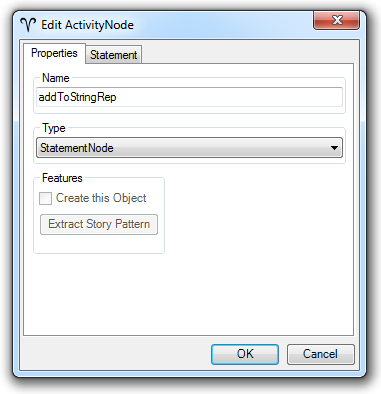
\includegraphics[width=0.5\textwidth]{ea_updateToStatement}
        \label{fig:updateStatement}
      }
      \subfloat[Edit the \texttt{MethodCallExpression} ]{
        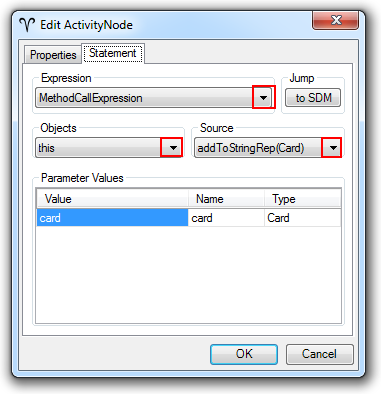
\includegraphics[width=0.5\textwidth]{ea_editStatementNode}
        \label{fig:editStatement}
      }
      \caption{}
\end{figure}
\FloatBarrier

\end{itemize}

Statement nodes should be used to interact with methods that are implemented by hand as they provide a means of invoking libraries and arbitrary Java code from
SDMs. Please note that we do not differentiate at this point between methods that are implemented via an SDM or by hand and thus, statement nodes can of course
be used to invoke other SDMs via a MethodCallExpression. Most importantly, this enables \emph{recursion} as the current SDM can be invoked on \texttt{this} with
appropriate new arguments.

\newpage

\begin{itemize}

\item[$\blacktriangleright$] To complete the SDM, return the final string representation value of the box via an \texttt{AttributeValueExpression} in
the stop node (Fig.~\ref{fig:toStringStopNode}).

\vspace{0.5cm}

\begin{figure}[htbp]
\begin{center}
  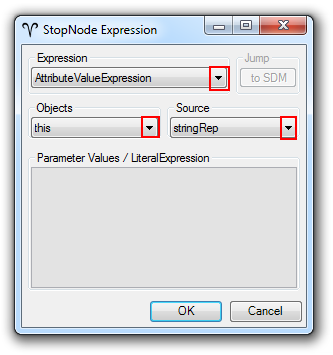
\includegraphics[width=0.5\textwidth]{ea_returnAttributeStopNode}
  \caption{Specify a return value}
  \label{fig:toStringStopNode}
\end{center}
\end{figure}

\vspace{0.5cm}

\item[$\blacktriangleright$] Take some time to compare and reflect on the complete SDM as depicted in Fig.~\ref{fig:sdm_tostring_5}.  The idea was to abstract
from the actual text representation of the box and model the necessary traversal of the data structure. The helper methods \texttt{addToStringRep} could, for example, build up a
string buffer and update this string representation. While modelling this SDM, we have seen that \emph{for each} stroy nodes can be nested, and have learnt two
new uses of MethodCallExpressions that provide a type safe\footnote{Apart from the literal expressions used for specifying argument values} means of invoking
methods from SDMs.

\vspace{0.5cm}

\item[$\blacktriangleright$] At this point, you should know the drill. Save, validate, and build your metamodel in Eclipse. To see how this is done in the
textual syntax, check out the nested loops in Fig.~\ref{fig:toStringFlow} and each pattern in Fig.~\ref{fig:toStringPatterns}

\newpage

\vspace*{2cm}

\begin{figure}[htbp]
\begin{center}
  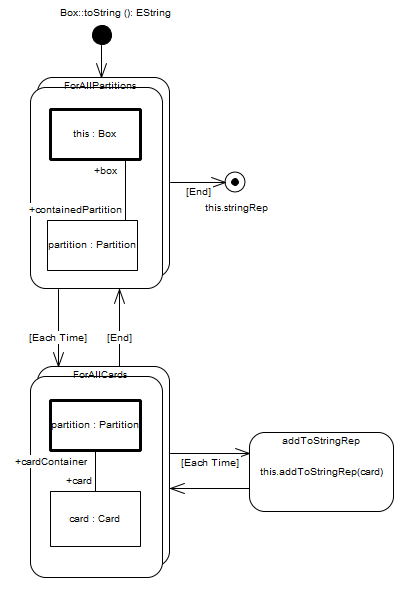
\includegraphics[width=0.8\textwidth]{ea_toStringComplete}
  \caption{The complete SDM for \texttt{Box::toString}}  
  \label{fig:sdm_tostring_5}
\end{center}
\end{figure}
\FloatBarrier

\jumpSingle{sec:fastCard}

\end{itemize}
